% Dies ist Teil der Vorlesung Physik auf dem Computer, SS 2012,
% Axel Arnold, Universitaet Stuttgart.
% 
% Dieses Werk ist unter einer Creative Commons-Lizenz vom Typ
% Namensnennung-Weitergabe unter gleichen Bedingungen 3.0 Deutschland
% zugänglich. Um eine Kopie dieser Lizenz einzusehen, konsultieren Sie
% http://creativecommons.org/licenses/by-sa/3.0/de/ oder wenden Sie sich
% schriftlich an Creative Commons, 444 Castro Street, Suite 900, Mountain
% View, California, 94041, USA.

\chapter{\keyword{Zufallszahlen}}
\index{Zufallszahlen>echte}

Im letzten Kapitel wurden für die Monte-Carlo-Integration
Zufallszahlen benötigt. In diesem Kapitel wird besprochen, wie diese
auf dem Computer generiert werden, welche Arten es gibt, und wie die
Qualität einer Zufallsreihe bestimmt werden kann. Außerdem lernen wir
weitere Anwendungen von Zufallszahlen kennen.

Zunächst aber klären wir, was Zufallszahlen im strengen Sinn sind. Wir
betrachten ein Experiment, dass wiederholt voneinander unabhängige
Ergebnisse $x \in M$ liefert.  Dann heißt ein Ergebnis einer solchen
Messung eine \emph{Zufallszahl}. Aufgrund der Konstruktion ist für
jede Zufallszahl $x$ der Erwartungswert gleich und unabhängig von
allen anderen Messungen. Betrachtet wir eine unendliche
Menge von Zufallszahlen, so sind die Zufallszahlen in dieser Menge
stets gleich verteilt, und zwar mit einer Verteilung $P(x)$, die durch
die Art des Experiments bestimmt ist.

Ein solches Experiment wäre zum Beispiel der Wurf eines Würfels, der
Ergebnisse aus $M=\{1,\ldots,6\}$ liefert. Ist dieser Würfel ideal, so
gilt $P(x) =\nicefrac{1}{6}$ für alle $x\in M$. Eine konkrete
Folge von Zufallszahlen wäre dann zum Beispiel
\begin{align*}
&633142563552446623663665614512446522561664446144244634522555 \\
&523121622535453613443366636251342661262345213346341313326554 \\
&221663665263462152654312621424115144626242451444653655341323\ldots
\end{align*}
und mit wachsender Folgenlänge würde der Anteil an Einsen, Zweien und
so weiter gegen jeweils $\nicefrac{1}{6}$ der Gesamtmenge
konvergieren.

Um echte Zufallszahlen bereitzustellen, müsste der Computer
vergleichbar ein (miniaturisiertes) Experiment mit bekannter,
stochastischer Verteilung der Messergebnisse durchführen. Wie Linux
zeigt, ist so etwas durchaus möglich, indem viele verschiedene
Hardwaredaten kombiniert werden, wie etwa Bits aus dem Netzwerkverkehr
oder der Mausposition. Diese Daten werden noch so transformiert, dass
sie gleichverteilte Bytes ergeben, die unter \texttt{/dev/random}
ausgelesen werden können. Wenn nichts weiter angegeben ist, wird auf
dem Computer übrigens üblicherweise von einer Gleichverteilung der
Zufallszahlen ausgegangen, also $P(x) = \nicefrac{1}{\abs{M}}$.

\section{\keyword{Pseudozufallszahlen}}
\index{Zufallszahlen>Pseudo-}

Für physikalische Anwendungen benutzt man allerdings keine echten
Zufallszahlen, sondern sogenannte \emph{Pseudozufallszahlen}. Dies
sind deterministische Zahlenfolgen, die aber "`hinreichend"' zufällig
aussehen; wir werden später sehen, was genau das
heißt. Pseudozufallszahlen haben zwei Vorteile. Zum einen lassen sich
solche Zahlen erheblich schneller berechnen als etwa die echten
Zufallszahlen des Linux-Kernels (um gut einen Faktor 80 auf modernen
Prozessoren), zum zweiten macht dies Computerexperimente exakt
reproduzierbar. Beobachtet man also bei einem Durchlauf ein
ungewöhnliches Verhalten, das man genauer analysieren möchte, kann man
das Experiment exakt wiederholen und dabei zum Beispiel zusätzliche
Messungen vornehmen.

Wie werden solche Pseudozufallszahlen generiert? Für diese Aufgabe
gibt es verschiedene Algorithmen, sogenannte
\emph{\keyword{Zufallszahlengeneratoren}} (engl. \emph{random number
  generator} oder \emph{RNG}). Diese liefern bei jedem Aufruf eine
Zufallszahl, meist eine gleichverteilte Ganzzahl. Die Bandbreite
reicht vom sehr guten, aber aufwändigen Mersenne-Twister bis zu den
einfachen linearen Kongruenzgeneratoren, die wir nun kennenlernen
werden.

Das Hauptmaß für die Güte eines solchen Zufallszahlengenerators ist
seine \emph{Periode}. Denn da jeder Zufallsgenerator einen internen
Zustand hat, der durch $N$ viele Bits dargestellt wird, muss sich nach
höchstens $2^N$ Aufrufen der interne Zustand wiederholen. Da es sich
aber um einen deterministischen Algorithmus handelt, wiederholt sich
die folgende Reihe ab dann exakt. Daher sind alle Generatoren
periodisch. Durch geeignete Wahl des Algorithmus ist die Periode meist
nahe dem theoretischen Maximum, also etwa $2^{32}\approx 4$ Milliarden
bei 32 Bit.

Das hört sich recht viel an, aber bei einer typischen
Molekulardynamiksimulation werden pro Zeitschritt und Teilchen 3
Zufallszahlen benötigt.  Bei zehntausend Teilchen werden damit pro
Schritt 30,000 Zufallszahlen gezogen, und der Generator wiederholt
sich nach weniger als 200,000 Zeitschritten. Da sich die
Teilchenpositionen in dieser Zeit wahrscheinlich schon stark geändert
haben, spielt dies in in der Praxis keine Rolle.  Bei Isingmodellen,
bei denen zufällig Spins auf einem Gitter invertiert werden,
betrachtet man allerdings nicht selten Gitter von einigen Millionen
Spins. In diesem Fall sind bessere Generatoren wesentlich.  Der
Mersenne-Twister-Generator hat zum Beispiel einen internen Zustand von
2,5 Kilobyte und eine Periode von $\approx 10^{6000}$, was für die
meisten Anwendungen ausreichend sein dürfte.

In Python stellt das Modul \texttt{random} verschiedene effiziente und
hochwertige Methoden zur Zufallszahlenberechnung bereit. Die Methode
\scipy{random.randint(a,b)} etwa liefert eine gleichverteilte
Zufallszahl aus dem Interval $[a,b]$; anders als bei \lstinline!range!
etwa ist also auch die obere Grenze
einbegriffen. \scipy{random.unifom(a,b)} liefert analog eine
gleichverteilte Fließkommazahl im Interval
$[a,b]$. \scipy{random.gauss(mu, sigma)} schließlich liefert eine
normalverteilte Fließkommazahl mit Erwartungswert \argd{mu} und
Standardabweichung \argd{sigma}.

NumPy hat ein eigenes \texttt{random}-Modul, das zusätzlich Vektoren
von Zufallszahlen generieren kann, indem einfach neben den Parametern
eine weitere ganze Zahl, die gewünschte Anzahl $N$ von Zufallszahlen,
angeben wird, also zum Beispiel \scipy{numpy.random.normal(mu, sigma,
  N)}. Achtung: anders beim \texttt{random}-Modul von Python ist bei
\scipy{numpy.random.randint(a, b, N)} \argd{b} \emph{nicht}
eingeschlossen!

\subsection{Linearer Kongruenzgenerator}
\index{Kongruenzgenerator>linearer}

Der (lineare) Kongruenzgenerator (LCG) ist der einfachste Typ eines
Zufallszahlengenerators. Der interne Zustand ist dabei lediglich eine
ganze Zahl $x_i$ von $0$ bis $m-1$, die gemäß
\begin{equation}
  x_{i+1} = a x_i + b \bmod m
\end{equation}
in den neuen inneren Zustand $x_{i+1}$ transformiert wird.  Die
eigentliche Zufallszahl sind einige (oder alle) der Bits des Zustands
$x_i$.  $m$, $a$ und $b$ sowie die Menge der für die Zufallszahl
benutzten Bits sind die Konstanten, die den Algorithmus festlegen,
$x_0$ der Startwert oder \emph{\keyword{Seed}}.  Die Konstanten $m$,
$a$ und $b$ sollten keinesfalls einfach zufällig gewählt werden, da
Knuth gezeigt hat, dass nur unter gewissen Bedingungen die Periode
eines solchen Generators tatsächlich $m$ ist~\cite{knuth81b}.  Bei
zufälliger Wahl der Konstanten wird die Periode meist sehr viel kürzer
sein.

Der Zufallsgenerator \texttt{rand48} der POSIX-C-Bibliothek ist ein
Beispiel eines LCGs.  Er benutzt einen Modul von $m=2^{48}$,
$a=25,214,903,917$ und $b=11$.  Als Zufallszahlen werden dann die
obersten 31 Bits von $x_i$ benutzt, also die Bits 17 bis 47.  Ältere
Versionen der Standard-C-Bibliothek benutzten für die Funktion
\texttt{rand} $m=2^{32}$, $a=1,103,515,245$ und $b=12,345$, wovon die
unteren 31 Bit als Zufallszahl genutzt werden.

Die Wahl von $m=2^{48}$ bzw. $m=2^{32}$ hat den einfachen Grund, dass
sich sehr einfach modulo $m=2^b$ rechnen lässt -- man berücksichtigt
einfach nur die ersten $b-1$ Bits und ignoriert alle höheren. Denn
\begin{equation}
  \label{eq:lcgmod}
  \left(\sum_{i=0}^\infty b_i 2^i\right) \bmod 2^b =
  \sum_{i=0}^\infty b_i \underbrace{\left(  2^i \bmod 2^b \right)}_{=
      0\,\text{für}\; i\ge b} \bmod 2^b = \sum_{i=0}^{b-1} b_i 2^i.
\end{equation}
Daher kann der klassische \texttt{rand} in C etwa wie folgt
implementiert werden:
\lstinputlisting[language=C,firstline=10]{rand.c}
Die Funktion \lstinline!rand_seed! dient zum Setzen des internen Zustands,
also $x_0$, \lstinline!rand! liefert dann bei jedem Aufruf eine neue
Zufallszahl.

Dass die Modulo-Operation für eine Zweierpotenz als Modul ein
einfaches Abschneiden der hohen Bits ist, hat allerdings auch einen
gewissen Nachteil.  Die ersten $k$ Bits der Zufallszahl bleiben beim
Abschneiden aller Bits $k+1,\ldots$ übrig.  Das bedeutet, dass diese
anscheinend von einem Generator mit kürzerer Periode $2^{k+1}$
generiert werden.  Insbesondere wechselt das unterste Bit mit jedem
Schritt seinen Wert oder ist konstant.  Dies ist der Grund, warum
\texttt{rand48} die untersten 17 Bit verwirft.

Dieses Problem lässt sich umgehen, in dem der Modul als Primzahl
gewählt wird. In diesem Fall kann $b=0$ gewählt werden, so dass
\begin{equation}
  x_{i+1} = a x_i = a^i x_0 \bmod m,
\end{equation}
wobei offenbar $x_0\neq 0$ sein muss. Wenn $a$ als eine primitive
Einheitswurzel des endlichen Körpers $\FF_m$ gewählt wird, dann
durchläuft diese Reihe einmal alle Elemente außer der Null. Daher hat
ein solcher Generator eine Periode von $m-1$.

$m$ wird meist als Mersennesche Primzahl, also von der Form $m=2^b -
1$, gewählt, wobei $b$ etwa so groß wie die Bitlänge des internen
Zustands ist. Dadurch ist die Periode des Generators nahezu maximal.
Die Implementation ist allerdings etwas schwieriger, weil jetzt die
oberen Bits nicht einfach abgeschnitten werden können. Nach Park und
Miller ist ein Beispiel eines solchen Generators $m=2^{31}-1$ und
$a=16807$, der auch als \texttt{MINSTD} bezeichnet wird und wie folgt
implementiert werden kann:
\lstinputlisting[language=C,firstline=10]{minstd.c}
Die Typumwandlung in \lstinline!long int! stellt dabei sicher, dass
das Produkt der beiden 32-Bit-Zahlen in 64-Bit-Arithmetik gerechnet
wird, so dass keine Stellen verloren gehen.

\subsection{Verzögerter Fibonaccigenerator}
\index{Fibonaccigenerator}
\index{Fibonaccigenerator>verzögerter}

Um eine längere Periode zu erzielen, könnte man im Prinzip zu immer
größeren Moduln $m$ übergehen. Allerdings wird es immer schwieriger,
entsprechende Konstanten zu bestimmen, und auch das Rechnung mit
Zahlen großer Bitlänge ist aufwändiger. Eine einfache Alternative
sind \emph{verzögerte Fibonaccigeneratoren}, die ähnlich wie ein LCG
funktionieren, aber mehrere vorherige Werte benutzen:
\begin{equation}
  x_n = x_{n-a} + x_{n-b} \bmod m,
\end{equation}
wobei diesmal $m$ beliebig ist und im allgemeinen einfach als die
Bittiefe des Rechners gewählt wird. Anstelle der Addition kann auch
die bitweise Addition modulo 2 benutzt werden.  Diese
Exklusiv-Oder-Operation war früher schneller als eine Addition und
wurde daher gern benutzt, bringt sonst allerdings eher Nachteile.  Der
interne Status des Zufallszahlengenerators besteht in diesem Fall aus
$\max(a,b)$ vielen $x_i$, die meist in einem
\emph{\keyword{Ringspeicher}} gespeichert werden.  Um diesen zu Anfang
zu füllen, benutzt man üblicherweise einen LCG, der nur einen
Startwert braucht.

Im Fall $a=b=1$ spricht man von einem Fibonaccigenerator, $a$ und $b$
sind ansonsten die Verzögerungen. Der Name stammt von den
Fibonaccizahlen, die ja der analogen Rekursion $x_n = x_{n-1} +
x_{n-2}$ genügen. Der Fibonaccigenerator selber, also $a=b=1$, ist
nicht sehr geeignet, gerade für den in der Physik häufigen Fall von
Dreierblöcken zeigt er unerwünschte Korrelationen.

Anders sieht es bei den verzögerten Fibonaccigeneratoren aus. Sofern
\begin{equation}
  x^a + x^b + 1
\end{equation}
ein primitives Polynom modulo zwei ist, also nicht faktorisierbar, hat
der verzögerte Fibonaccigenerator eine Periodenlänge von mindestens
$2^a-1$. Um einen 32-Bit-LCG an Periodenlänge zu übertreffen,
sind also wenigstens 32 Registerplätze im Ringspeicher nötig. Stoll
und Kirkpatrick geben als Parameter $a=250$, $b=103$ an, eine andere
mögliche Kombination ist $a=521$, $b=168$.

\begin{figure}
  \centering
  \begin{tikzpicture}[thick, x=0.95\textwidth,y=\baselineskip]
    \newcommand{\mycount}{10}%
    \newcommand{\myfirst}{21}%
    \newcommand{\mysecond}{24}%
    \pgfmathsetmacro{\mywidth}{1.0/\mycount}
    
    \draw (1.3*\mywidth, 2) node[anchor=west] {$p = 1$} ;
    \draw[very thick, ->]
    (1.5*\mywidth, 1.5) --
    (1.5*\mywidth, 1) ;

    \draw (4.3*\mywidth, 2) node[anchor=west] {$p + 10 - 7 \bmod 10 = 4$} ;
    \draw[very thick, ->]
    (4.5*\mywidth, 1.5) --
    (4.5*\mywidth, 1) ;

    \draw (2.3*\mywidth, -5) node[anchor=west] {$p' = 2$} ;
    \draw[very thick, ->]
    (2.5*\mywidth, -4.5) --
    (2.5*\mywidth, -4) ;

    \pgfmathsetmacro{\last}{\myfirst + \mycount-1}%
    \foreach \idx in {\myfirst,...,\last} {
      \pgfmathsetmacro{\x}{mod(\idx - 20 + \mycount,
        \mycount)*\mywidth}
      \ifthenelse{\equal{\idx}{\myfirst}}{
        \draw[fill=green!50!white] (\x,0) rectangle +(\mywidth, 1);
      }{}
      \ifthenelse{\equal{\idx}{\mysecond}}{
        \draw[fill=blue!50!white] (\x,0) rectangle +(\mywidth, 1);
      }{}
      \draw (\x,0) rectangle +(\mywidth, 1);
      \draw (\x + 0.5*\mywidth, 0.5) node {$x_{\idx}$};
    }

    \draw (2.5*\mywidth, -1.5) node {$x_{n} = x_{n-10} + x_{n-7}$} ;
    \draw[very thick, dotted, ->]
    (1.5*\mywidth, 0) --
    (1.5*\mywidth, -0.5) --
    (2.5*\mywidth, -0.5) --
    (2.5*\mywidth, -1) ;
    \draw[very thick, dotted, ->]
    (4.5*\mywidth, 0) --
    (4.5*\mywidth, -0.5) --
    (3.5*\mywidth, -0.5) --
    (3.5*\mywidth, -1) ;
    \draw[very thick, dotted, ->] (1.5*\mywidth, -2) -- (1.5*\mywidth, -3) ;

    \renewcommand{\myfirst}{22}%
    \renewcommand{\mysecond}{25}%
    \newcommand{\mylast}{31}%
    \pgfmathsetmacro{\last}{\myfirst + \mycount-1}%
    \foreach \idx in {\myfirst,...,\last} {
      \pgfmathsetmacro{\x}{mod(\idx - 20 + \mycount, \mycount)*\mywidth}
      \ifthenelse{\equal{\idx}{\mylast}}{
        \draw[fill=red!50!white] (\x,-4) rectangle +(\mywidth, 1);
      }{}
      \ifthenelse{\equal{\idx}{\myfirst}}{
        \draw[fill=green!20!white] (\x,-4) rectangle +(\mywidth, 1);
      }{}
      \ifthenelse{\equal{\idx}{\mysecond}}{
        \draw[fill=blue!20!white] (\x,-4) rectangle +(\mywidth, 1);
      }{}
      \draw (\x,-4) rectangle +(\mywidth, 1);
      \draw (\x + 0.5*\mywidth, -3.5) node {$x_{\idx}$};
    }
  \end{tikzpicture}
  
  \caption{Illustration eines Ringspeichers für $b=10$ Werte. $p$ gibt
    die aktuelle Position des ältesten Elements im Ringspeicher an, im
    Beispiel steht an Stelle $p=1$ der Wert $x_{21}$. Das neueste
    Element ist $x_{30}$, daher wollen wir $x_{31}=x_{21} + x_{24}$
    berechnen. $x_{21}$ befindet sich gerade an der Stelle $p$,
    $x_{24}$ dementsprechend $10-7 = 3$ Positionen weiter rechts,
    wobei Positionen jenseits des rechten Randes links wieder
    hereinlaufen. Im nächsten Schritt ist dann $p=2$, und das zweite
    Element an der Stelle 4. Die Folgenwerte sind also wie auf einem
    Ring gespeichert.}
  \label{fig:ringspeicher}
\end{figure}

In Code sieht ein einfacher verzögerter Fibonaccigenerator so aus:
\lstinputlisting[language=C,firstline=10]{r250.c}
Abbildung~\ref{fig:ringspeicher} illustriert dabei die Funktion und
Indizierung des Ringspeichers.

\section{Andere Verteilungen}

Die bisher besprochenen Zufallszahlengeneratoren liefern stets ganze
Zahlen in einem gewissen Intervall, \texttt{rand48} zum Beispiel
im Intervall $[0,2^{31}-1]$, \texttt{MINSTD} im Intervall
$[1,2^{31}-1]$. Um daraus gleichverteilte Ganzzahlverteilungen in
beliebigen Intervallen zu erzeugen, kann man die Zufallszahl einfach
skalieren. Ist also $\xi$ eine Zufallszahl, die gleichverteilt aus
$[a,b]$ gezogen wird, so ist
\begin{equation}
  \xi' = \frac{\xi - a}{b-a}
\end{equation}
gleichverteilt in $[0,1]$ und umgekehrt
\begin{equation}
  \xi'' = a' + \frac{(b'-a')(\xi - a)}{b-a}
\end{equation}
gleichverteilt in $[a',b']$. Dabei muß bei Ganzzahlarithmetik zuerst
multipliziert und dann dividiert werden, da $\xi' \le 1$. Zusätzlich
ist $b$ meist knapp an der Bitlänge der Architektur, daher muss das
Produkt mit doppelter Bitzahl berechnet werden. Da die Prozessoren,
die zum wissenschaftlichen Rechen benutzt werden, meist auch sehr
schnell Fließkommazahlen verarbeiten, kann alternativ auch $\xi'$ in
in Fließkommadarstellung berechnet werden und daraus $\xi''$. Soll
$\xi''$ ganzzahlig sein, kann es dabei einfach gerundet werden. Diesen
Weg benutzt zum Beispiel Python. Auf diese Weise können natürlich auch
(pseudo-)zufällige gleichverteilte Fließkommazahlen erzeugt werden,
insbesondere \emph{Standardzufallszahlen}\index{Standardzufallszahl},
also Fließkommazahlen im Bereich $[0,1]$.

Wie aber können nun etwa normalverteilte Zufallszahlen erzeugt werden?
Hierfür lernen wir nun mehrere Verfahren kennen, die
Standardzufallszahlen in im Prinzip beliebige andere Verteilungen
umwandeln.

\subsection{\keyword{Verwerfungsmethode}}
\index{Rejection sampling}

Angenommen, wir wollen Zufallsvektoren gleichverteilt aus einer
Kreisscheibe vom Radius $1$ ziehen, d.~h.~, wir wollen Zufallsvektoren
$p=(x,y)$ ziehen, die gemäß der Dichte
\begin{equation}
  \rho(x, y) = \begin{cases}
    \nicefrac{1}{\pi} & \text{für}\; x^2+y^2\le 1\\
    0     & \text{sonst}
  \end{cases}
\end{equation}
verteilt sind.  Abbildung~\ref{fig:pi} links zeigt, wie man dies
bewerkstelligen könnte: man zieht zunächst zwei unabhängig
gleichverteilte Zufallszahlen auf $[-1,1]$ und interpretiert diese als
Koordinaten $p = (x, y)$. Liegt $p$ in der Kreisscheibe, akzeptieren
wir dies als unseren Zufallsvektor, ansonsten versuchen wir es einfach
erneut. Da die Wahrscheinlichkeit, gezogen zu werden, für alle
Kreisscheibenpunkte gleich ist, sind die zurückgelieferten $p$
gleichverteilt. Als Code sieht dies so aus:
\begin{lstlisting}
from numpy.random import uniform

def kreisscheibe():
    while True:
        x = uniform(-1, 1)
        y = uniform(-1, 1)
        if x**2 + y**2 <= 1:
            return (x, y)
\end{lstlisting}
Da wir im Mittel nur $1-\pi/4$ der gezogenen Punkte benutzen, brauchen
wir $\nicefrac{4}{(4-\pi)}$ mal mehr Zufallszahlen, als wir als
Koordinaten der Punkte zurückliefern. Im Falle des Kreises ist der
Verlust nicht sehr hoch, aber ist die zulässige Struktur kleiner,
können sehr viele Zufallszahlen zurückgewiesen werden, und die
Verwerfungsmethode wird ineffizient.

\begin{figure}
  \centering
  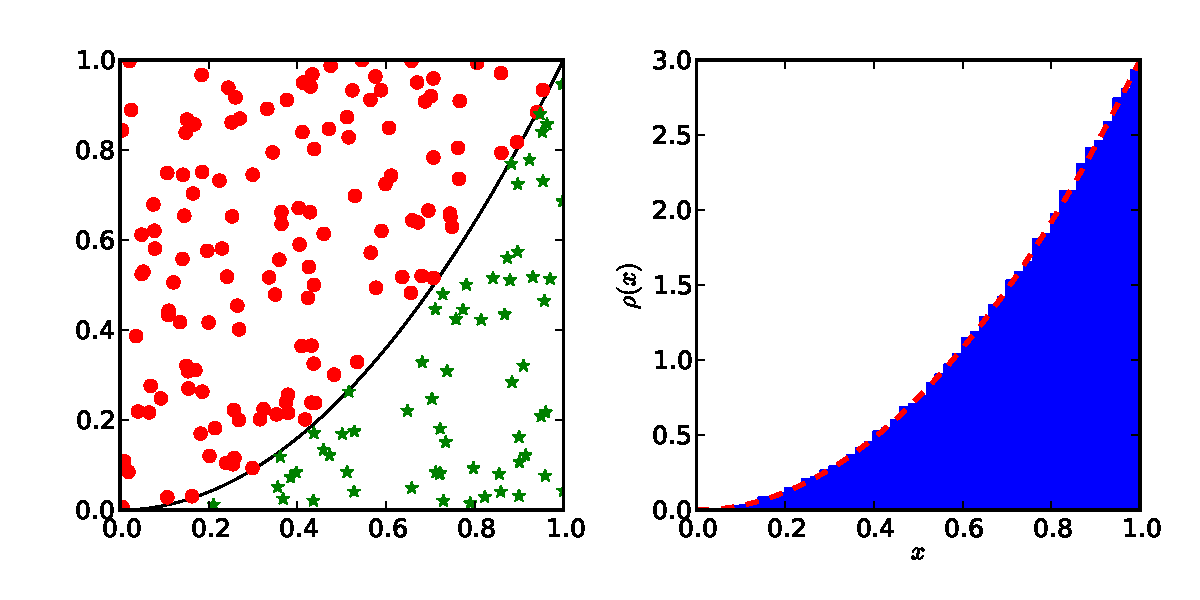
\includegraphics[width=\textwidth]{plots/rejection}
  \caption{Verwerfungsmethode zur unnormierten Verteilung
    $\rho(x)=x^2$ für $0\le x \le 1$. Links sind einige gezogene
    Punkte eingezeichnet, von denen die grünen Sterne akzeptiert
    wurden, die roten Kreise abgelehnt. Der schwarze Strich stellt
    $\rho(x)$ dar. Rechts sind die beobachteten Häufigkeiten der
    Punkte als Balken dargestellt. Diese stimmen gut mit der
    normierten Dichte $3x^2$ überein, die rot gestrichelt
    eingezeichnet ist. Hier werden im Schnitt etwa drei Zufallszahlen
    pro Aufruf der Verwerfungsmethode benötigt.}
  \label{fig:rejection}
\end{figure}

Im Falle der Kreisscheibe war die Dichte $\rho(x, y)$ der gesuchten
Verteilung sehr einfach, nämlich entweder $0$ oder $1/\pi$. Die
Verwerfungsmethode lässt sich aber auch bei komplizierteren $\rho$
anwenden. Wir betrachten nun eine Dichte $\rho:\RR^n\to [0,1]$, so
dass $\rho$ außerhalb $[0,1]^n$ Null ist. Dann müssen die Punkte $p$
mit relativen Wahrscheinlichkeiten $\rho(p)$ gezogen werden. Das lässt
sich einfach bewerkstelligen, indem wir zunächst einen Punkt $p$ durch
Ziehen von $n$ Standardzufallsvariablen gleichverteilt in $[0,1]^n$
bestimmen. Wir ziehen nun eine weitere Standardzufallszahl $u$ und
akzeptieren $p$ nur dann, wenn $u\le\rho(p)$. Die Wahrscheinlichkeit,
$p$ tatsächlich zu ziehen, ist dann
\begin{equation}
  P(u \le\rho(p)) = \rho(p).
\end{equation}

Die korrekte Wahrscheinlichkeit für einen Punkt $p$ im Würfel ist die
infinitesimale Dichte $\rho(p)\,dx^n$. Da der Normierungsfaktor $dx^n$
für alle $p$ gleich ist, können wir diesen vernachlässigen, da die
relativen Wahrscheinlichkeiten auf $[0,1]^n$ trotzdem korrekt
sind. Das bedeutet auch, dass die Eingabe-"`Dichte"' $\rho(p)$ gar nicht
normiert sein muss --- die Verwerfungsmethode liefert stets
Ergebnisse, die gemäß der normierten Dichte
\begin{equation}
  \tilde\rho(p) := \rho(p) / \int_{[0,1]^n} \rho(q)\,dq^n
\end{equation}
verteilt sind. Damit können auch Dichten behandelt werden, die nicht
in $[0,1]$ liegen, so lange sie beschränkt sind, denn man kann in
diesem Fall
\begin{equation}
  \rho'(p) = \frac{\rho(p) + \min_{p\in [0,1]^n} \rho(p)}{
    \max_{p\in [0,1]^n} \rho(p) - \min_{p\in [0,1]^n} \rho(p)} \in [0,1]
\end{equation}
betrachten. Die Normierungseigenschaft ist auch sehr günstig, wenn die
Normierungskonstante nicht einfach bestimmt werden kann, etwa bei sehr
hochdimensionalen Räumen. Dies ist die Grundlage des
Metropolissampling, dass eine zentrale Rolle in der numerischen
statistischen Physik spielt. Abbildung~\ref{fig:rejection} illustriert
die Verwerfungsmethode und ihre Normierungseigenschaft.

Im Falle der Kreisscheibe hatten wir übrigens auch von der
Normierungseigenschaft Gebrauch gemacht, denn eigentlich ist $\rho(p)$
Null außerhalb der Kreisscheibe und $\nicefrac{1}{\pi}$ innerhalb. Da
wir aber die Punkte innerhalb automatisch akzeptiert haben, haben wir
formal ein $\rho'$ betrachtet mit $\rho'(p) = 1$ auf der
Kreisscheibe. Dank der Normierungseigenschaft haben wir damit trotzdem
die korrekte Verteilung erzeugt.

Als Python-Code sieht die allgemeinere Verwerfungsmethode nicht
wesentlich schwieriger aus:
\begin{lstlisting}
from numpy.random import uniform

def verwerfungsmethode(rho, n):
    while True:
        p = uniform(0, 1, n)
        u = uniform(0, 1)
        if u < rho(p):
            return p
\end{lstlisting}
\argd{rho} muss dabei eine Pythonfunktion sein, die als einziges
Argument ein $n$-dimensionales Numpy-Array akzeptiert.

Die Verwerfungsmethode kann so erweitert werden, dass die benutzten
Zufallszahlen  nicht gleichverteilt sind, sondern etwa
normalverteilt. Das erlaubt, die Verwerfungsmethode auch bei über dem
gesamten $\RR^n$ nichtverschwindenden Dichten zu benutzen. Siehe
hierzu zum Beispiel \textcite{knuth81b}. Wie man solche
normalverteilten Zufallszahlen erzeugt, lernen wir nun kennen.

\subsection{\keyword{Inversionsmethode}}

Wegen der Beschränkung auf einen Würfel können wir die
Verwerfungsmethode nicht benutzen, um zum Beispiel normalverteilte
Zufallszahlen aus gleichverteilten zu generieren. Wir benötigen also
noch eine andere Methode, um auch unbeschränkte Verteilungen erzeugen
zu können. Hier bietet sich die Inversionsmethode an.

Sei $\rho:\RR\to \RR$ eine normierte Wahrscheinlichkeitsdichte, zu der
wir passend Zufallszahlen ziehen wollen. Dann definieren wir die
Verteilungsfunktion zu $\rho$ als
\begin{equation}
  F_\rho(x) := P(u_\rho \le x) = \int_{-\infty}^{x} \rho(x')\, dx',
\end{equation}
wobei $u_\rho$ eine $\rho$-verteilte Zufallszahl ist.  $F_\rho(x)$
gibt also die Wahrscheinlichkeit an, einen Wert kleiner als $x$ zu
beobachten, und bildet daher die reelle Achse monoton wachsend in das
Intervall $[0,1]$ ab. Das $p$-Quantil ist nun die Umkehrung
$F_\rho^{-1}(p)$, also diejenige Grenze $x$, bei der ein gezogener
Wert mit Wahrscheinlichkeit $p$ kleiner als $x$ ist. Es gilt also
\begin{equation}
  F_\rho\left(F_\rho^{-1}(p)\right) = p.
\end{equation}

$F_\rho^{-1}(u)$ ist eine $\rho$-verteilte Zufallsvariable, wenn $u$
eine Standardzufallszahl ist, also gleichverteilt auf $[0,1]$. Denn
\begin{equation}
  P(F_\rho^{-1}(u) \le x) = P(u \le F_\rho(x)) = F_\rho(x).
\end{equation}
Sofern also die Quantilfunktion einfach zu invertieren ist, lassen
sich so sehr bequem Zufallszahlen erzeugen, indem $F_\rho^{-1}$ auf
Standardzufallszahlen angewendet wird.

\subsubsection{\keyword{Box-Muller-Verfahren}}

\begin{figure}
  \centering
  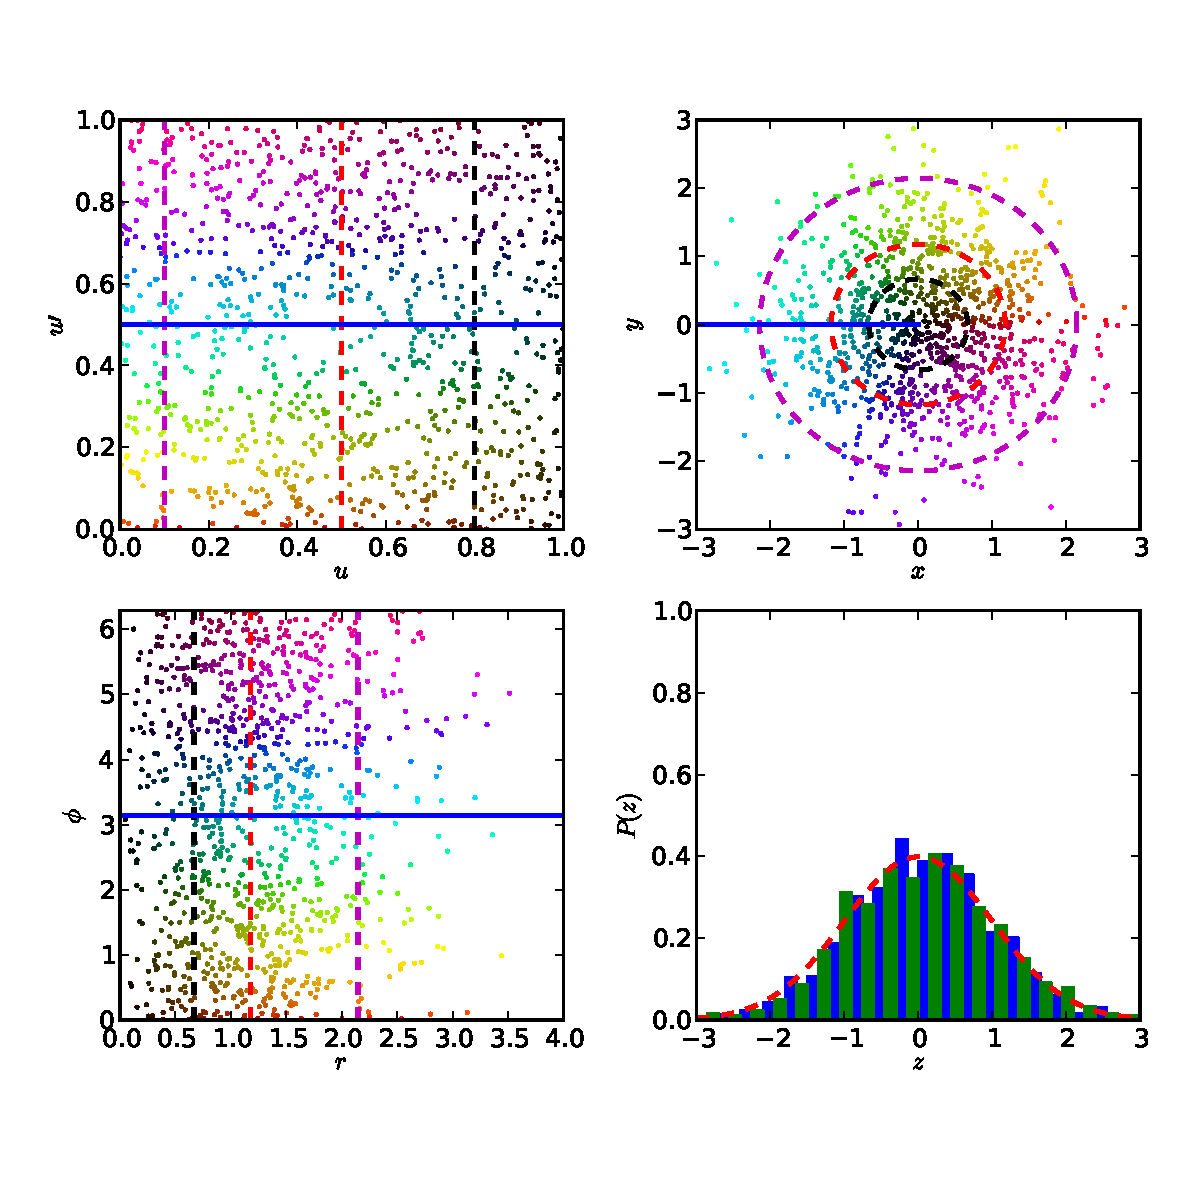
\includegraphics[width=\textwidth]{plots/inversion}
  \caption{Illustration des Box-Muller-Verfahrens zur Erzeugung von
    normalverteilten Zufallszahlen. Die Punkte werden zunächst
    gleichverteilt auf $[0,1]^2$ erzeugt (links oben), dann
    gemäß \eqref{eq:expquantil} auf das Gebiet
    $[0,\infty)\times[0,2\pi]$ transformiert (links unten), und
    schließlich in kartesische Koordinaten (rechts oben). Die Punkte
    sind in allen drei Graphen stets gleich gefärbt, und zwar mit
    wechselnder Farbe im Winkel und sinkender Intensität nach
    außen. Rechts unten sind die gemessenen Verteilungen von $x$ und
    $y$ sowie die erwartete Gaußverteilung gezeigt.}
  \label{fig:boxmuller}
\end{figure}

Mit Hilfe der Inversionsmethode können wir nun auch normalverteilte
Zufallszahlen erzeugen. Allerdings nicht auf direktem Wege, da das
Integral der Gaußfunktion, die Fehlerfunktion, nicht einfach
analytisch zu invertieren ist. Box und Muller gehen daher ähnlich wie
bei der Bestimmung des uneigentlichen Integrals von $e^{-x^2}$ vor
und weichen auf zwei Dimensionen aus.

Wir betrachten also einen Zufallsvektor $(x, y)$ mit Dichte $\rho(x,
y) = \frac{1}{2\pi}e^{-\frac{1}{2}(x^2 + y^2)}$. In Polarkoordinaten
$(\phi,r)$ transformiert diese Dichte zu
\begin{equation}
  \rho(\phi, r) = \frac{1}{2\pi}e^{-\frac{1}{2}r^2} r.
\end{equation}
Wir benötigen also einen gleichverteilten Zufallswinkel $\phi\in
[0,2\pi]$, sowie einen Abstand $r\in [0,\infty)$ mit Dichte $\rho_r(r)
= e^{-\frac{1}{2}r^2} r$. Die zugehörige Verteilungsfunktion ist
\begin{equation}
  F_{\rho_r}(r) = \int_0^r e^{-\frac{1}{2}s^2} s\, ds = 1 - e^{-\nicefrac{r^2}{2}},
\end{equation}
dessen Umkehrung, also das $p$-Quantil,
\begin{equation}
  \label{eq:expquantil}
  F_{\rho_r}^{-1}(p) = \sqrt{-2\log(1 - p)}.
\end{equation}
Da, falls mit $p$ auch $p-1$ gleichverteilt auf $[0,1]$ ist, ergibt
sich durch Rücktransformation in kartesische Koordinaten das
Box-Muller-Verfahren als
\begin{align}
  x  = \sqrt{-2\log(u)}\cos(2\pi u')\\
  y = \sqrt{-2\log(u)}\sin(2\pi u')
\end{align}
mit zwei Standardzufallszahlen $u$, $u'$. Diese werden in zwei
unabhängige, normalverteilte Zufallszahlen $z$ und $z'$
transformiert. Anders als bei der Verwerfungsmethode erhält man also
genauso viele normalverteilte Zufallszahlen wie gleichverteilte
verbraucht werden, allerdings müssen diese immer paarweise erzeugt
werden. Abbildung~\ref{fig:boxmuller} illustriert die Anwendung der
Inversionsmethode zur Erzeugung normalverteilter Zufallszahlen.

\subsection{Zufällige Punkte auf Kugel und Kugeloberfläche}

Wie wir bereits gesehen haben, lassen sich mit Hilfe der
Verwerfungsmethode gleichverteilt Positionen in der Kreisscheibe
ziehen, und analog natürlich auch Positionen aus jeder Kugel im
$\RR^n$. Allerdings nimmt die Akzeptanzrate mit steigendem $n$ rasch
ab, da die $n$-Kugel nur noch einen kleinen Teil von $[-1,1]^n$
belegt. Bis etwa $n=4$ ist die Verwerfungsmethode allerdings sehr
effizient, was für die meisten physikalischen Anwendungen reicht.

Sollen Punkte auf der Kugeloberfläche gezogen werden, so können diese
im Prinzip aus über der Kugel gleichverteilten Punkten $p$ gewonnen
werden, indem diese auf die Oberfläche projiziert werden, also
$p/\norm{p}$ betrachtet. Allerdings benötigt man auf diese Weise $n$
Zufallszahlen, um einen Zufallsvektor auf der nur $n-1$-dimensionalen
Oberfläche zu generieren, zusätzlich zu den Verlusten durch die
Verwerfungsmethode. Daher ist es im Einzelfall besser, eine geschickte
Parametrisierung der Oberfläche zu nutzen.

Für die Oberfläche der zweidimensionalen Kugel, also den Kreis, ist
dies sehr einfach, da dieser über einen Winkel $\phi\in [0,2\pi]$
gleichmäßig parametrisiert wird. Wird also eine Standardzufallszahl
$u$ gezogen, so sind die Punkte
\begin{equation}
  \begin{split}
    x &= r\sin(2\pi u)\\
    y &= r\cos(2\pi u)
  \end{split}
\end{equation}
gleichverteilt auf einem Kreis vom Radius $r$ um Null.

Für die Oberfläche der dreidimensionalen Kugel, also die 2-Sphäre, ist
nicht etwa die gebräuchliche Parametrisierung über zwei Winkel am
besten, sondern die Parametrisierung in Zylinderkoordinaten $\phi$ und
$z$.  Der Winkel $\phi$ ist offenbar gleichverteilt und kann als $2\pi
u$ bestimmt werden, wobei $u$ eine Standardzufallsvariable ist.  $z$
ist erstaunlicherweise ebenso gleichverteilt, da $\rho(z)$
proportional zum Flächeninhalt des jeweiligen Rings ist, dividiert
durch den gesamten Flächeninhalt, also
\begin{equation}
  \rho(z) = \frac{1}{4\pi r^2} 2\pi \sqrt{r^2 - z^2} \sqrt{1 +
    \left(\frac{d}{dx}\sqrt{r^2 - z^2}\right)^2} = \frac{1}{2r}
\end{equation}
für $-r\le z\le r$.

Um eine gleichverteilte Position auf der Kugeloberfläche zu ziehen,
genügt es daher, zwei Standardzufallszahlen $u$ und $u'$ zu
berechnen, und diese gemäß
\begin{equation}
  \label{eq:2sphere}
  \begin{split}
    z &= r(2u' - 1)\\
    y &= \sqrt{r^2-z^2}\cos(2\pi u)\\
    x &= \sqrt{r^2-z^2}\sin(2\pi u)
  \end{split}
\end{equation}
zu transformieren.

\section{Qualitätsanalyse}
\index{Pseudozufallszahlen>Qualitätsanalyse}

Um die Qualität eines Zufallszahlengenerators zu testen, gibt es eine
Vielzahl von Standardtests. Der Grund dafür ist, dass es leider keinen
einzelnen Test gibt, der sicherstellt, dass es keinerlei Korrelationen
in der generierten Folge gibt. Ein solcher Test müßte jede mögliche
Teilmenge bilden und mit allen Zahlen korrelieren, was praktisch nicht
möglich ist. Daher sollte ein guter Zufallszahlengenerator möglichst
viele der folgenden Tests erfüllen, auch wenn dies keine Garantie ist,
dass er im Einzelfall nicht doch zu kritischen Korrelationen führt,
die im schlimmsten Fall das Ergebnis beieinflussen.

Für eine bestimmte Anwendung genügt es natürlich, wenn er nur die
Tests erfüllt, deren getestete Korrelationen Einfluß auf das System
haben. Zum Beispiel werden bei einer Molekulardynamiksimulation in
drei Dimensionen Paarkorrelationen unwichtig sein, aber
Tripletkorrelationen problematisch.  Bei einem zweidimensionalen
Isingmodell hingegen wird es genau umgekehrt sein.  In jedem Fall aber
sollte die Periode des Generators wie besprochen groß genug sein.

Für die im folgenden beschriebenen Tests nehmen wir an, dass der zu
testende Zufallszahlengenerator Standardzufallszahlen liefert, also
gleichverteilt im Intervall $[0,1]$.  Solche Zufallszahlen werden wie
beschrieben standardmäßig auf dem Computer erzeugt und im Bedarfsfall
auf andere Verteilungen transformiert.

\subsubsection{Statistiktests}
\index{$\chi^2$-Test}

\begin{figure}
  \centering
  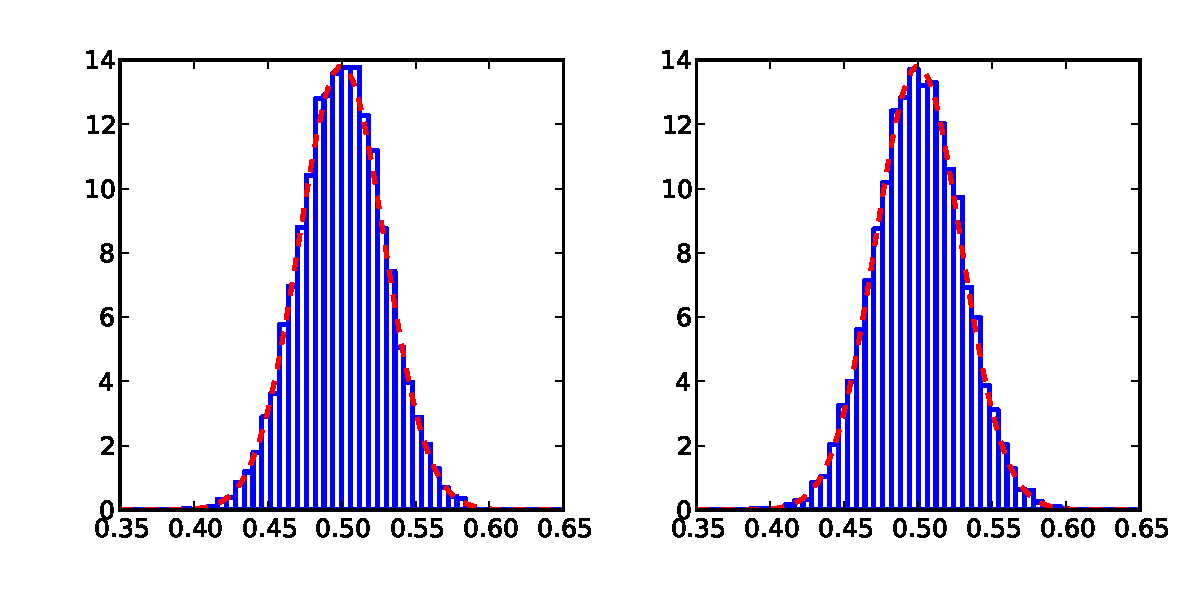
\includegraphics[width=\textwidth]{plots/statistics_test}
  \caption{Verteilung von $\overline{x} = \sum_{i=1}^{100} x_i$,
    ermittelt aus 20,000$\times$100 Werten der Zufallsgeneratoren
    \texttt{rand} (links) und \texttt{minstd} (rechts). Rot
    gestrichelt ist jeweils die erwartete Normalverteilung mit Varianz
    $\nicefrac{1}{\sqrt{1200}}$ eingezeichnet.}
  \label{fig:statistics_test}
\end{figure}

Sind die erzeugten Zufallszahlen $x_i$ tatsächlich gleichverteilt auf
$[0,1]$, so gilt für den Mittelwertschätzer
\begin{equation}
  \mean{\overline{x}} =
  \mean{\frac{1}{N} \sum_{i=1}^N x_i}
  = \mean{x} = \frac{1}{2}
\end{equation}
und für dessen Varianz nach \eqref{eq:esterr}
\begin{equation}
  \sigma(\overline{x}) = \frac{1}{\sqrt{N}} \sigma(x) =
  \frac{1}{\sqrt{12 N}}.
\end{equation}
Für immer größere $N$ sollte daher $\overline{x}$ gegen
$\nicefrac{1}{2}$ konvergieren.

Wird $\overline{x}$ sehr oft für disjunkte Zufallszahlenmengen $\{x_i,
i=1(1)N\}$ gemessen, so sollte $\overline{x}$ außerdem für große $N$
gemäß dem Gesetz der großen Zahlen praktisch normalverteilt sein, mit
der oben angegebenen Varianz. Dies kann mit Hilfe von
\eqref{eq:varest} überprüft werden, man kann aber auch direkt das
Histogram der Verteilung von $\overline{x}$ darauf überprüfen, dass es
wie erwartet normalverteilt ist.  Abbildung~\ref{fig:statistics_test}
zeigt die Verteilung von $\overline{x}$ am Beispiel von
\texttt{MINSTD} und \texttt{rand}, sowie die erwartete
Normalverteilung.  Diese Art von Test wird auch als $\chi^2$-Test
bezeichnet.

\subsubsection{Poincar\'e-Schnitte}
\index{Würfeltest}\index{Quadrattest}

\begin{figure}
  \centering
  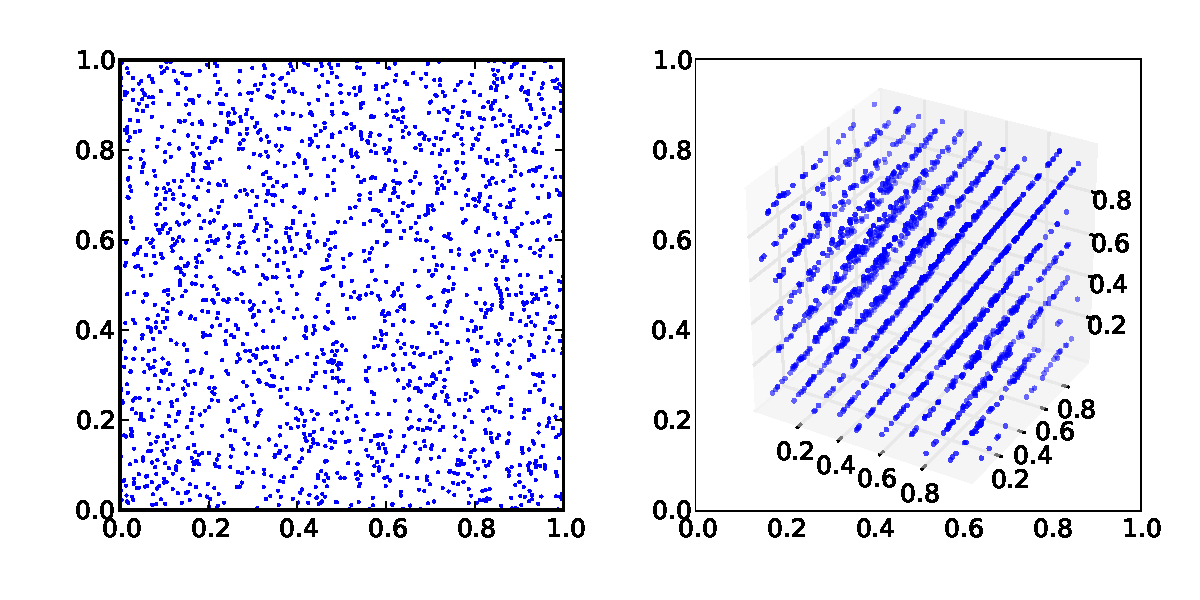
\includegraphics[width=\textwidth]{plots/optical_test}
  \caption{Quadrat- und Würfeltest mit 2,000 Auswertung am Beispiel
    des berüchtigten \texttt{RANDU}-Zufallszahlengenerators. Der
    zweidimensionale Poincar\'e-Schnitt ist homogen und unauffällig,
    aber in drei Dimensionen fallen die nur sehr wenigen Hyperebenen
    des Generators deutlich auf.}
  \label{fig:optical_test}
\end{figure}

Lineare Kongruenzgeneratoren haben nach einem Satz von Marsaglia die
Eigenschaft, dass im $\RR^n$ $n$ aufeinanderfolgende Zufallszahlen,
als Vektor aufgefasst, auf Hyperebenen liegen. Problematisch wird
dies, wenn die Anzahl der Hyperebenen sehr klein ist. Für $n=2$ und
$3$ kann man das sehr bequem überprüfen, in dem man den
Poincar\'e-Schnitt $(x_k, x_{k+1})$, $k=0,1,\ldots$ bzw. sein
dreidimensionales Äquivalent $(x_k, x_{k+1}, x_{k+2})$, $k=0,1,\ldots$
betrachtet. Da alle Punkte in $[0,1]^2$ bzw $[0,1]^3$ liegen, heißen
dieses Tests auch Quadrat- oder Würfeltests. Diese Punktwolken sollten
das Quadrat bzw. den Würfel homogen füllen und keine Strukturen
aufweisen. In zwei Dimensionen können wir das sehr rasch erfassen, in
drei Dimensionen muss man die Punktewolke rotieren, um nach
Hyperebenen zu suchen.

Abbildung~\ref{fig:optical_test} demonstriert dies für den
berüchtigten \texttt{RANDU}-LCG ($m=2^{31}$, $a=65,539$,
$b=0$). Dieser ist wegen des $2^{31}$-Moduls sehr schnell auf
32-Bit-Rechnern zu implementieren und war daher früher sogar auf
einigen Großrechnern zu finden. In der zweidimensionalen Darstellung
sind keine Auffälligkeiten zu sehen, aber ausgerechnet in den
physikalisch wichtigen drei Dimensionen zeigt sich, dass es lediglich
eine Handvoll verschiedener Hyperebenen gibt, so dass mit diesem
Generator erzeugte 3d-Vektoren kaum als zufällig gelten können.

\subsubsection{\keyword{Fouriertest}}
\index{Spektraltest}

\begin{figure}
  \centering
  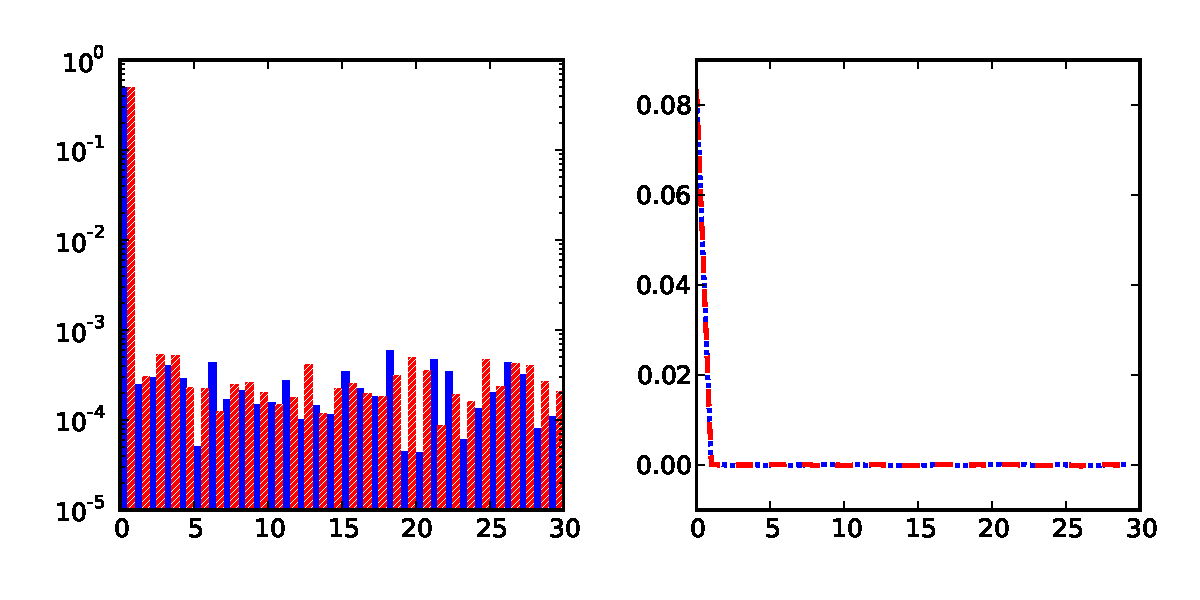
\includegraphics[width=\textwidth]{plots/fft_tests}
  \caption{Spektraltest (links) und Autokorrelationsfunktion (rechts)
    für die Zufallszahlengeneratoren \texttt{rand} und
    \texttt{MINSTD}. \texttt{rand} ist als blaue Fläche bzw. gepunktet
    eingezeichnet, \texttt{MINSTD} rot gestrichelt.  Im linken Graph
    sind die DFT-Amplituden normiert dargestellt, also dividiert durch
    die Anzahl der Zufallszahlen, so dass die 0-te Mode $1/2$ beträgt.}
  \label{fig:fft_tests}
\end{figure}

Wird eine lange Reihe von Standardzufallszahlen diskret
Fourier-transformiert, so sollte die 0-te Mode eine Amplitude von
$N/2$ aufweisen, da diese ja die Summe der Zufallszahlen angibt. Alle
anderen Moden sollten vernachlässigbar kleine, gleichmässige
Amplituden haben, entsprechend einem weißen Rauschen. Die Amplituden
aller Frequenzen ungleich $0$ sollte außerdem mit der Länge der
transformierten Zufallszahlenreihe sinken. Dieser Test wird auch als
Spektraltest bezeichnet. Abbildung~\ref{fig:fft_tests} zeigt die
DFT am Beispiel von \texttt{rand} und \texttt{MINSTD}.

\subsubsection{\keyword{Autokorrelationstest}}

Neben der diskreten Fouriertransformierten kann man auch die
Autokorrelationsfunktion der Zufallsreihe $u$ bestimmen, also
\begin{equation}
  C(u,u)(k) = \frac{1}{N}\,\text{iDFT}
  \bigl(\overline{\text{DFT}(u)(n)}\,\text{DFT}(u)(n)\bigr)(k).
\end{equation}
Für eine Zufallsreihe sind alle paarweise verschiedenen Werte
unkorreliert, also muss
\begin{equation}
  C(u,u)(k) = \sigma^2(u)\delta_k = \frac{1}{12}\delta_k
\end{equation}
gelten. Dies ist in Abbildung~\ref{fig:fft_tests} rechts
demonstriert.

\section{Beispiel: \keyword{Random walk}}

\begin{figure}
  \centering
  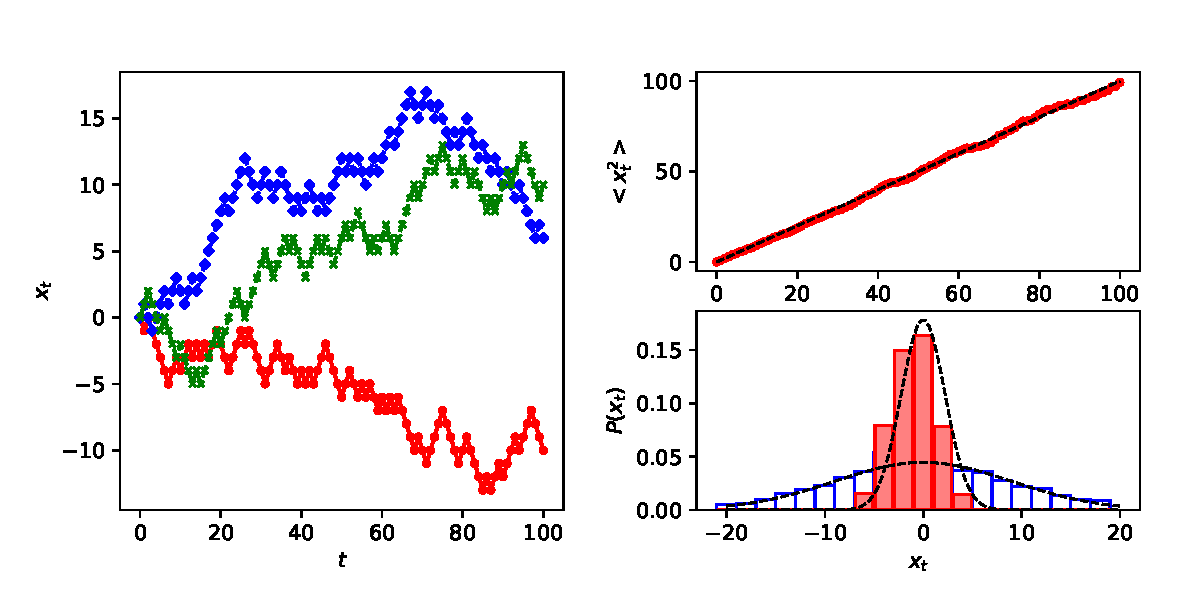
\includegraphics[width=\textwidth]{plots/rw}
  \caption{Links: 3 mögliche Random walks gemäß \eqref{eq:rw}, als
    Funktion der Zeit $t$. Rechts oben ist das mittlere
    Verschiebungsquadrat als Funktion der Zeit gezeigt, gemittelt über
    1000 Random walks. Die gestrichelte Linie markiert dabei das
    analytisch erwartete Ergebnis $\mean{x_T^2}=T$. Rechts unten
    die Verteilungen der Positionen zu den Zeitpunkten $t=5$ (rote,
    gefüllte Balken) und $t=80$ (blaue, offene Balken). Gestrichelt sind
    wieder die jeweils erwarteten Normalverteilungen eingezeichnet.}
  \label{fig:rw}
\end{figure}

Als Beispiel für die Anwendung von Zufallszahlen in der physikalischen
Simulation soll der Randomwalk ("`Irrfahrt"') dienen, der in vielen
Problemen der statistischen Physik eine Rolle spielt. Das klassische
Beispiel ist die Brownsche Bewegung von Partikeln in Wasser oder
anderen Flüssigkeiten. Diese wird durch die unzähligen Stöße der
Lösungsmittelmoleküle auf das betrachtete Teilchen erklärt.

Hat das betrachtete Teilchen einen Durchmesser von nur 1$\mu$m, so
befinden sich an seiner Oberfläche zu jedem Zeitpunkt ca. eine halbe
Milliarde Lösungsmittelmoleküle. Deren Bewegung explizit simulieren zu
wollen, ist aussichtslos. Auf der anderen Seite passieren selbst in
kurzer Zeit genügend Zusammenstöße, so dass die zeitdiskretisierte
Kraft auf das Teilchen gut als zufällig und, wegen des Gesetzes der
großen Zahlen, normalverteilt angenommen werden kann. Der Mittelwert
ist dabei offenbar Null, da die Zufallsstöße keine Vorzugsrichtung
haben sollten, die Varianz werden wir mit der Diffusionskonstanten in
Verbindung bringen.

Um diesen Prozess zu simulieren, können wir uns zunächst auf ein
eindimensionales Modell beschränken, da die Stöße in den
einzelnen Koordinaten unabhängig sind. Indem wir das Gesetz der großen Zahl
andersherum anwenden, können wir außerdem eine beliebige, aber
symmetrische Verteilung der Stöße annehmen. Die einfachste Möglichkeit
ist, einfach mit gleicher Wahrscheinlichkeit dieselbe Distanz vor-
oder zurückzugehen.

Wir betrachten also ein Teilchen mit Position $x_t$ zum Zeitpunkt
$t=1, 2,\ldots$, so dass
\begin{equation}
  \label{eq:rw}
  x_{t+1} = x_t +
  \begin{cases}
    -1 & \text{mit Wahrscheinlichkeit \nicefrac{1}{2}}\\
    +1 & \text{mit Wahrscheinlichkeit \nicefrac{1}{2}}.
  \end{cases}
\end{equation}

Ein \emph{Random walk} ist eine Folge $x_t$, die durch eine solche
einfache stochastische Bewegungsgleichung beschrieben wird.
Abbildung~\ref{fig:rw} zeigt links drei mögliche solche Random
walks. Sie wurden durch eine Routine ähnlich der folgenden generiert: 
\begin{lstlisting}
def rw(N):
    x = 0
    xt = [ x ] 
    for move in randint(0,2,N):
        if   move == 0: x += -1
        elif move == 1: x +=  1
        xt.append(x)
    return xt
\end{lstlisting}

Dieses Modell ist so einfach, dass wir seine statistischen
Eigenschaften fast vollständig analytisch berechnen können. So ist zum
Beispiel
\begin{equation}
  \mean{x_t} = \mean{\sum_{s=1}^{t} u_s} = 0, 
\end{equation}
wobei $u_{s} = x_{s} - x_{s-1}$ den $s$-ten Schritt des Random walks
bezeichnet, und daher $\mean{u_s} = 0$ gilt. Die mittlere Position des
Random walks bleibt also stets am Ausgangspunkt. Allerdings wird die
Verteilung der Punkte $x_t$ mit $t$ immer breiter, denn für das
mittlere Verschiebungsquadrat gilt
\begin{equation}
  \label{eq:sigmarw}
  \mean{x_t^2} =
  \mean{\sum_{s,r=1}^{t} u_su_r} = \sum_{s=1}^{t}\mean{u_s^2}
  = t\sigma^2(u_s) = t.
\end{equation}
Für hinreichend große $t$ kennen wir damit auch die
Wahrscheinlichkeitsdichte der Positionen, die gemäß dem Gesetz der
großen Zahlen praktisch Gaußsch ist:
\begin{equation}
  \rho(x, t) = \rho(x_t) \approx \frac{1}{\sqrt{2\pi\sigma^2}}
  \exp\left(-\frac{x_t^2}{2\sigma^2}\right).
\end{equation}
Die Varianz ist dabei $\sigma^2 = \sigma^2(x_t) = \mean{x_t^2}$, also
das mittlere Verschiebungsquadrat.

Abbildung~\ref{fig:rw} zeigt rechts oben das mittlere
Verschiebungsquadrat $\sigma^2(x_t)$, gemittelt über 1,000 Random
walks. $\sigma^2(x_t)$ ist tatsächlich mit guter Genauigkeit ungefähr
$t$, wobei die Abweichung für große $t$ größer sind, da dort die
Verteilung von $x_t$ breiter ist, und damit auch der Fehlerbalken der
Varianz. Rechs unten werden für $t=5$ und $t=80$ die Verteilungen der
Positionen gezeigt. Selbst für $t=5$ werden diese gut durch die
Gaußglocke beschreiben.  Trotzdem sollte man sich erinnern, dass die
Verteilung nicht wirklich Gaußsch ist, da offenbar $\abs{x_t}\le t$
gilt. Denn der maximale Abstand ist erreicht, wenn wir $t$-mal nur
nach links oder rechts gehen. Während also die Gaußverteilung
prinzipiell beliebig hohe Werte mit sehr kleiner Wahrscheinlichkeit
zulässt, ist die tatsächliche Verteilung beschränkt.

Das Modell lässt sich leicht auf mehrere Dimensionen erweitern, denn
die Zufallsbewegungen in den einzelnen Koordinaten sind ja
unabhängig. Die mittlere Position des Random walks in $n$ Dimensionen
ist damit immer noch konstant gleich der Ausgangsposition, das
mittlere Verschiebungsquadrat die Summe der Verschiebungsquadrate der
Koordinaten, also $\mean{x_t^2} = n t \sigma^2(u)$, wobei
$\sigma^2(u)$ das Verschiebungsquadrat der einzelnen Dimensionen
bezeichnet.

\subsubsection{Diffusion}

Was ist nun die Bedeutung von der Konstanten $D=\sigma^2(u) =
\sigma^2(x_t)/t$?  Wir verallgemeinern den Random walk, der bisher in
Zeit um $\Delta t=1$ und Raum um $\pm\Delta x = \pm 1$ gesprungen ist,
auf beliebige Werte $\Delta x$ und $\Delta t$. Dann gilt offenbar $D =
\sigma^2(u) = \Delta x^2/\Delta t$. Wir betrachten nun die
Master-Gleichung der diskreten Wahrscheinlichkeitspopulationen
\begin{equation}
  \Delta p(x, t + \Delta t) = p(x, t + \Delta t) - p(x, t) =
  \frac{1}{2}p(x - \Delta x, t) +
  \frac{1}{2}p(x + \Delta x, t) - p(x, t).
\end{equation}
Die erste Term der rechten Seite besagt, dass das Teilchen beim Sprung
$t\to t +\Delta$ mit Wahrscheinlichkeit $\frac{1}{2}$ an der Stelle
$x$ landet, wenn es sich zum Zeitpunkt $t$ an der Stelle $x-\Delta x$
befand. Der darauffolgende Term bedeutet dasselbe für $x+\Delta$, und
der letzte Term, dass das Teilchen nicht an der aktuellen Stelle
bleiben kann.

\begin{figure}
  \centering
  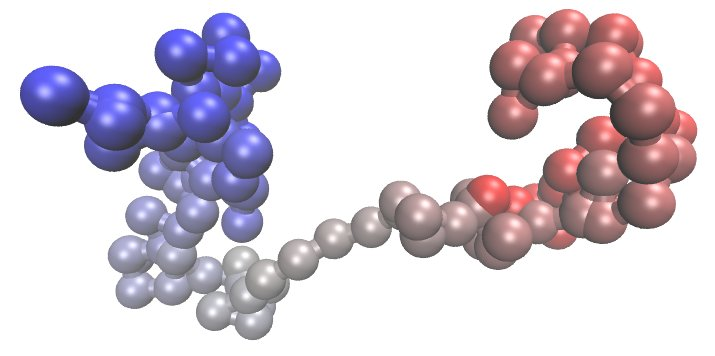
\includegraphics[width=0.6\textwidth]{plots/polymer}
  \caption{Kontinuierlicher Random walk als einfaches Polymermodell mit
    $n=100$ Monomeren. Das Polymer wurde mit der Simulationssoftware
    \textsc{ESPResSo}~\cite{espresso} erzeugt und dem
    Visualisierungstool \texttt{VMD}~\cite{vmd} gezeichnet.}
  \label{fig:contrw}
\end{figure}

Wir multiplizieren nun linker Hand mit $\Delta t^{-1}$ und rechter Hand mit
$\Delta x^{-2}$:
\begin{equation}
  \frac{\Delta p(x, t + \Delta t)}{\Delta t} =
  \frac{D}{2\Delta x^2} \left(p(x - \Delta x, t) +
    p(x + \Delta x, t) - 2 p(x, t)\right).
\end{equation}
Lassen wir nun $\Delta t\to 0$ und $\Delta x\to 0$ gehen, wird aus
dieser Gleichung die Differentialgleichung
\begin{equation}
  \frac{\delta p}{\delta t} p(x, t) =
  D\frac{\delta^2 p}{\delta x^2} p(x, t).
\end{equation}
Dies ist nichts anderes als die Diffusionsgleichung mit
Diffusionskonstante $D$. Die Varianz $D=\sigma^2(u)$ unseres
Zufallsschritts ist also genau die Diffusionskonstante unserer
makroskopischen Teilchen, und durch geeignete Wahl von $\sigma^2(u)$
können wir die Diffusionskonstante unserer Random walk-Teilchen
einstellen.

\subsubsection{Random walks als Polymermodell}
\index{Random walk>kontinuierlicher}

Man kann für den mehrdimensionalen Random walk leicht zeigen, dass es
keinen wesentlichen Unterschied macht, wenn die nächsten Positionen
nicht diskret $\pm 1$ in allen Dimensionen gewählt werden, sondern zum
Beispiel kontinuierlich oder auf einer Sphäre, d.h.,
\begin{equation}
  x_{t+1} = x_t + u \quad\text{mit}\; \norm{u}=1,\,u\text{ gleichverteilt}.
\end{equation}
Ein solcher kontinuierlicher Random walk kann mit Hilfe von
\eqref{eq:2sphere} leicht numerisch erzeugt werden, ein Beispiel ist
in Abbildung~\ref{fig:contrw} gezeigt.

Die letztere Wahl ist ein einfaches Modell für Polymere unter
bestimmten Voraussetzungen (in einem sogenannten
$\theta$-Lösungsmittel).  In diesem Fall ist $t$ allerdings keine
Zeitachse, sondern zählt einfach die Monomere entlang der Polymerkette
durch.

In guten Lösungsmitteln streckt sich das Polymer etwas mehr. Auch dies
lässt sich durch einen Random walk modellieren, bei dem die Monomere
eine endliche Ausdehnung haben und nicht überlappen können. Ein
solcher Random walk heißt auch \emph{Self avoiding walk}, weil er sich
selbst nicht kreuzen kann. In unserem einfachen Random walk-Modell
\eqref{eq:rw} entspricht das der Bedingung $x_t\neq x_s$ für alle
$s\neq t$ und ist auf dem Computer relativ einfach zu erstellen.

Um einen Self avoiding walk zu generieren, erzeugt man einfach einen
Random walk, und überprüft mit jedem neuen Punkt, ob dieser einem
anderen Monomer näher kommt als die Größe der Monomere zulässt. In
diesem Fall muss man allerdings ganz von vorne beginnen, da sonst
extrem ungünstige Konfigurationen bevorzugt werden. Bei diesen würde
ja quasi beliebig lange probiert, den nächsten Punkt zu setzen, selbst
wenn es nur eine verschwindend geringe Wahrscheinlichkeit gibt, diesen
Punkt zufällig zu treffen. Daher werden taschenartige Konfigurationen
sehr viel wahrscheinlicher, als sie zufällig auftreten würden. Ab etwa
100 Monomeren ist die Wahrscheinlichkeit, einen Random walk
abzulehnen, schon sehr hoch, und die Erzeugung eines Self avoiding
walks dementsprechend aufwändig.

Auch von der Theorie her ist der Self avoiding walk sehr viel
komplizierter. So gilt etwa $\mean{x_N^2} \sim N^{2\nu}$ mit
$\nu\approx 0.588$, so dass das Polymer im Mittel tatsächlich etwas
mehr gestreckt ist als der Random walk mit $\nu=\nicefrac{1}{2}$. Der
Wert von $\nu$ für den Self avoiding walk kann, anders als beim Random
walk, nicht analytisch berechnet werden, sondern nur aufwändig
numerisch genähert.

Der Self avoiding walk wie auch der der einfache Random walk spielen
nach wie vor eine wichtige Rolle in der Polymerphysik, insbesondere
beim Aufsetzen von Polymersimulationen. Daher besitzt etwa
Simulationssoftware \textsc{ESPResSo}~\cite{espresso} einen eigenen
Befehl, um solche Zufallsketten zu erzeugen.

\subsubsection{Diffusionslimitierte Aggregation}

\begin{figure}
  \centering
  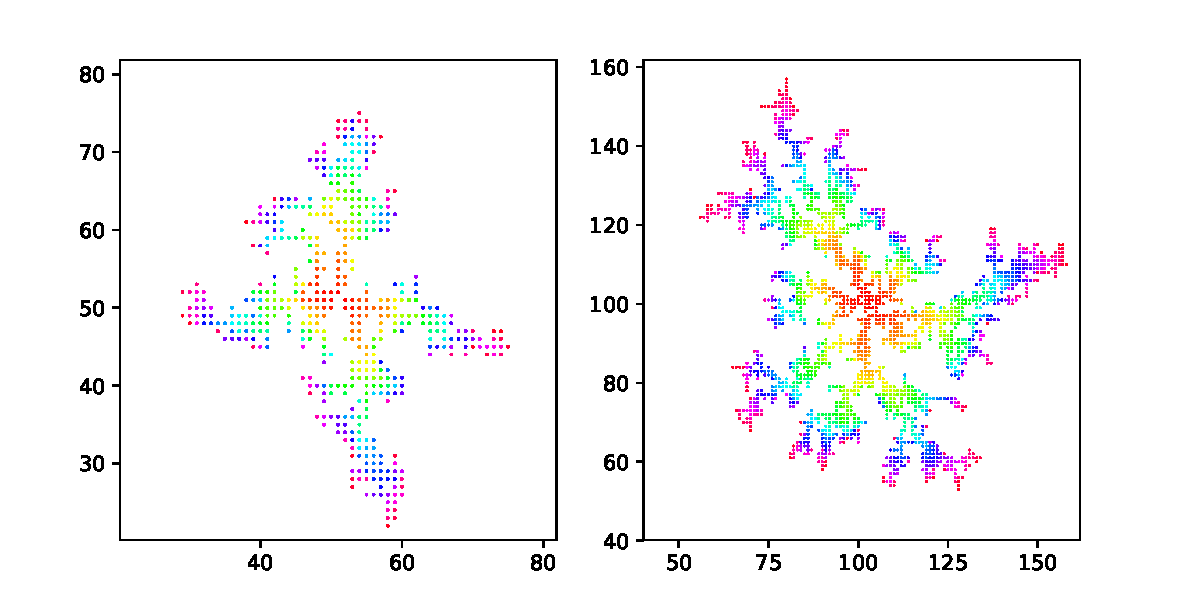
\includegraphics[width=\textwidth]{plots/dla}
  \caption{Cluster aus diffusionslimitierter Aggregation mit $N=500$
    (links) und $N=2000$ (rechts) Teilchen. Die Teilchen sind in der
    Reihenfolge der Anlagerung farblich codiert.}
  \label{fig:dla}
\end{figure}

Eine weitere Anwendung des Random walks ist die diffusionslimitierte
Aggregation, die etwa die Bildung von Rußaggregaten modelliert. Dabei
wird davon ausgegangen, dass sich diese aus einem Keim durch
Anlagerung von weiteren Teilchen bilden, die aus dem Unendlichen heran
diffundieren.

Für die Modellierung werden Random walks genutzt, die zufällig auf
einer Kugelsphäre um den Keim gestartet werden, bis sie entweder am
Cluster anlagern oder sich zu weit vom Kreis entfernt
haben. Abbildung~\ref{fig:dla} zeigt zwei solche DLA-Cluster mit 500
und 2000 Teilchen auf einem zweidimensionalen Gitter. Die beiden
Cluster haben eine sehr ähnliche Struktur, auch wenn die Maßstäbe
deutlich anders sind. Das hängt damit zusammen, dass solche
diffusionslimitierte Aggregate selbstähnliche Fraktale
sind. Listing~\ref{lst:dla} zeigt den Python-Code zur Erzeugung
solcher zweidimensionaler DLAs.

Die zentrale Frage beim Studium von DLA-Clustern ist die nach ihrer
fraktalen Dimension. In drei Dimensionen legen wir zu ihrer Bestimmung
konzentrische Kugeln mit Radius $R$ um den Keim eines sehr großen
Clusters, und zählen die Anzahl der Teilchen $N(R)$ in dieser
Kugel. Die fraktale Dimension ist dann
\begin{equation}
  d = \lim_{R\to\infty}\frac{\log N(R)}{\log R}.
\end{equation}
In der Praxis betrachtet man natürlich einfach mehrere große Cluster
verschiedener Größe, um $d$ abzuschätzen.  Wäre der Cluster solide mit
Teilchendichte $\rho$, so wäre $N(R) = \rho \frac{4\pi}{3} R^3$ und
\begin{equation}
  \frac{\log N(R)}{\log R} = \frac{\log\left( \rho
      \frac{4\pi}{3} R^3\right)}{\log R} =
  3 + \frac{\log\left( \rho\frac{4\pi}{3}\right)}{\log R},
\end{equation}
die fraktale Dimension also wie erwartet 3. Der DLA-Cluster in drei
Dimensionen hat übrigens eine fraktale Dimension von $\approx 1,6$,
ist also bei weitem kein solides Objekt. Daher werden solche Cluster
gerne als Katalysatoren verwendet, da sie eine entsprechend große
Oberfläche haben.

\raggedbottom \lstinputlisting[style=multipage, firstline=10,
caption={Code zur
  Erzeugung eines DLA-Clusters auf einem zweidimensionalen Gitter
  \argd{world}. Die Eingabeparameter sind die Größe \argd{M} des
  Gitters, sowie die Anzahl der Punkte des zu erzeugenden Aggregats
  \argd{N}. Das Aggregat entsteht durch sukzessive Anlagerung mit
  Hilfe von Random walks, die auf einem langsam wachsenden Kreis um
  das aktuelle Aggregat starten. Der Radius \argd{R} diese Kreises ist
  stets um 5 Gittereinheiten größer als der Umkreis des Clusters.},
label=lst:dla]{dla.py}

\section{Beispiel: \keyword{Perkolation}}

Ein anderes Beispiel eines Zufallsalgorithmus ist die Perkolation,
also die Frage, wann ein Zufallsmedium einen durchgehenden Kanal
zulässt oder nicht. Anwendungsbeispiele sind etwa poröse Medien, die
Flüssigkeiten nur passieren lassen, falls es einen durchgehenden
Hohlraum gibt, oder eine Mischung von Isolator und Leiter, die nur
leitet, wenn es eine leitende Verbindung gibt.

Modellieren lässt sich dies als ein Gitter, dessen Zellen mit einer
gewissen Wahrscheinlichkeit $p$ besetzt sind. Die Frage ist dann, ab
welcher kritischen Wahrscheinlichkeit $p_c$ es im Regelfall einen
Cluster von benachbarten, besetzten Feldern gibt, der das gesamte
System in einer Richtung durchzieht, man sagt,
\emph{perkoliert}. Diese Grenze lässt sich durch Untersuchen sehr
vieler zufälliger Besetzungen untersuchen.

Die Besetzungen sind dabei natürlich durch stochastisches Belegen des
Gitters sehr einfach zu erzeugen, algorithmisch etwas schwieriger ist
nur, zu bestimmen, ob es einen perkolierenden Cluster gibt, also
einen, der eine Seite mit der gegenüberliegenden verbindet.

Eine Möglichkeit ist, die Struktur von einer Seite aus gewissermaßen
zu "`fluten"', und zu sehen, ob man dabei die gegenüberliegende Seite
erreicht. Erreichen heißt hier, dass es einen zusammenhängenden Pfad
von paarweise benachbarten, besetzten Punkten gibt. Um dies zu
überprüfen, erzeugen wir zunächst eine Liste der besetzten Punkte am
Start\-rand.  Dann fügen wir zu dieser Liste alle benachbarten Punkte
hinzu, und wiederholen dies solange, bis keine neuen Elemente mehr zur
Liste hinzugefügt wurden. Die Liste enthält dann alle Punkte, die
Verbindung zum Startrand haben. Wir müssen nur noch überprüfen, ob in
dieser Liste Punkte am gegenüberliegenden Rand auftauchen.

\begin{figure}
  \centering
  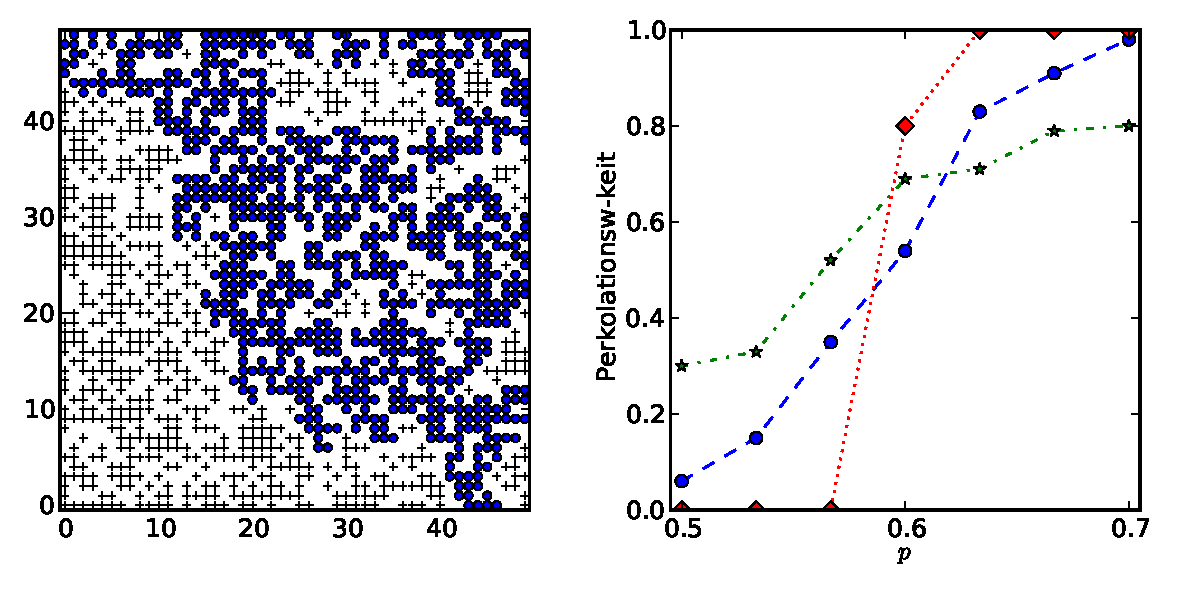
\includegraphics[width=\textwidth]{plots/percolation}
  \caption{Ein perkolierender Cluster auf einem $50^2$-Gitter mit
    $p=0,6$. Blaue Punkte markieren den Cluster, Kreuze andere, mit
    diesem Cluster nicht verbundene, aber besetzte Gitterpunkte. Im
    rechten Graph ist für $L=5$ (grüne Sterne), $L=20$ (blaue
    Diamanten) und $L=100$ mit welcher Wahrscheinlichkeit bei
    Besetzung $p$ ein perkolierender Cluster gefunden wurde. Für
    $L=100$ ist dies ein bereits sehr scharfer 0--1-Übergang in Nähe
    von $0,6$.}
  \label{fig:percolation}
\end{figure}

In dieser Form wäre der Algorithmus recht langsam, weil man ständig
wieder Punkte hinzufügen würde, die bereits in der Liste sind, und
diese erneut untersucht. Um dies zu vermeiden, führt man einfach eine
zweite Liste der Punkte, deren Nachbarn noch nicht untersucht
wurden. Ein Punkt, der noch nicht in der Liste der verbunden Punkte
steht, wird dann nicht nur zu dieser, sondern auch zur Liste der zu
bearbeitenden Punkte hinzugefügt. Dann müssen nur die Nachbarn der
Punkte in dieser Liste betrachtet werden, und sobald die Nachbarn
eines Punkts einmal untersucht wurden, kann dieser aus der Liste der
zu bearbeitenden Punkte gestrichen werden. Da er aber immer noch als
verbunden markiert ist, wird er auch nie ein zweites Mal in die Liste
der zu bearbeitenden Punkte eingefügt werden. Der Algorithmus
terminiert also, da die abzuarbeitende Liste irgendwann leer ist. Ein
entsprechendes Python-Skript ist in Listing~\ref{lst:percolation} zu
sehen.

Abbildung~\ref{fig:percolation} zeigt links einen perkolierenden
Cluster für ein Gitter mit Besetzungwahrscheinlichkeit $p=0,6$, es
sind also etwas mehr als die Hälfte der Punkte besetzt. Rechts ist für
verschiedene Besetzungswahrscheinlichkeiten aufgetragen, wie
wahrscheinlich es ist, einen perkolierenden Cluster zu beobachten. Wie
man sieht, ist $p=0,6$ nicht ohne Grund gewählt, denn dies ist sehr
dicht am kritischen Perkolationsschwellwert. Der tatsächliche Wert des
Schwellwerts ist $p_c\approx 0,593$ im Limit unendlicher Gittergröße,
wie man zeigen kann. Mit steigender Kantenlänge wird der Übergang
bereits bei endlichen Gittern relativ scharf, bei $L=100$ ist der
Grenzbereich weniger als $0,06$ in $p$ breit. Bei einer Besetzung von
$0,56$ ist Perkolation äußerst unwahrscheinlich, bei $0,6$ gibt es
hingegen schon für die Mehrheit der Gitter einen perkolierenden
Cluster.

Ähnlich wie beim Random walk kann auch die Perkolation in unzähligen
Variationen betrachtet werden, etwa andere zugrundeliegende Gitter,
höhere Dimensionen oder auch kontinuierliche Modelle.

\afterpage{
\raggedbottom \lstinputlisting[style=multipage,firstline=10,
caption={Code zur Schätzung des Perkolationsschwellwerts auf einem
  zweidimensionalen quadratischen Gitter \argd{world}. Die Liste
  \argd{connected} enthält die alle Punkte, die mit dem oberen Rand
  verbunden sind, die Liste \argd{connected_undone} diejenigen
  verbundenen Punkte, deren Nachbarn noch untersucht werden
  müssen.}, label=lst:percolation]{percolation.py}
}
%%% Local Variables: 
%%% mode: latex
%%% TeX-master: "padc"
%%% TeX-PDF-mode: t
%%% End: 
